\documentclass{article}

\usepackage{graphicx}
\usepackage{subcaption}
\usepackage{amsmath}
\usepackage{amsfonts}

\begin{document}

\author{Zachary Vogel}
\date{\today}
\title{Notes in APPM 4650\\Adam Norris}

\maketitle



\section{2nd Project}
\begin{figure}[h!]
    \centering
    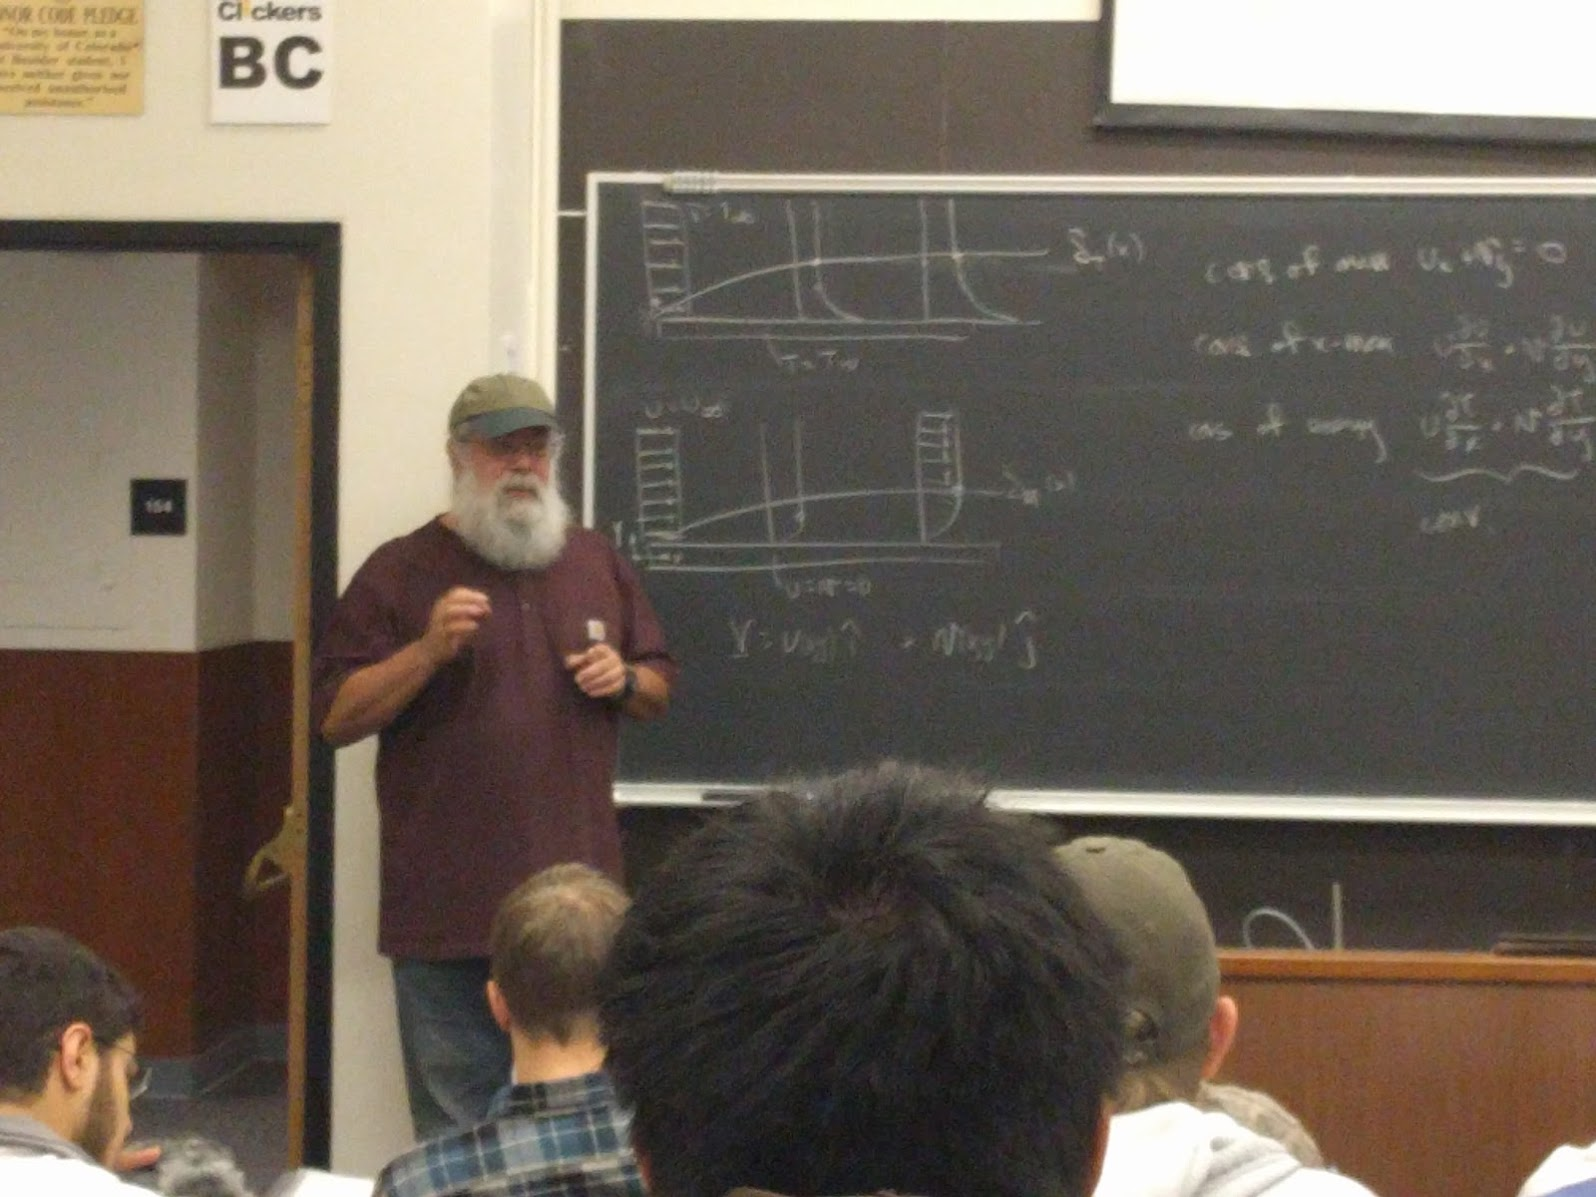
\includegraphics[width=0.8\textwidth]{proj21.jpg}
\end{figure}
conservation of mass $u_x+\mathfrak{v}_y=0$.\\
conservation of x-momentum $u\frac{du}{dx}+\mathfrak{v}\frac{du}{dy}=\nu\frac{d^2u}{dy^2}$\\
conservation of energy $u\frac{d\tau}{dx}+\mathfrak{v}\frac{dT}{dy}=\alpha\frac{d^2T}{dy^2}$\\
first 2 terms are convection and last is diffusion.\\
$v=u(x,y)\hat{i}+\mathfrak{v}(x,y)\hat{j}$ u is horizontal and v is vertical.\\
$T(x,y)$ need this and $u(x,y)$ and $\mathfrak{v}(x,y)$\\

highest order x derivative of u is 1, $x=0\ u=u_\infty$\\
highest order y derivative of u is 2, $y=0\ u=0$, $y\to\infty\ u\to u_\infty$\\

highest order v derivative with respect to x is 0\\
highest order v derivative with respect to y is 1, $y=0\ v=0$\\

highest order T derivative with respect to x is 1, $x=0\ T=T_\infty$\\
highest order T derivative with respect to y is 2, $y=0\ T=T_\infty$\\
and $y\to\infty\ T=T_\infty$\\

\[\eta=\cfrac{y}{\sqrt{\cfrac{\nu x}{u_\infty}}}\]
\[F(\eta)=f(\eta)\]
\[u=u_\infty F'(\eta)\]
\[\mathfrak{v}=\cfrac{1}{2}\sqrt{\cfrac{\nu u_\infty}{x}}(\eta F'(\eta)-F(\eta))\]
\[G=\cfrac{T-T_\infty}{T_\omega-T_\infty}=G(\eta,Pr)\]
Pr is the Prendel number $Pr=\frac{\nu}{\alpha}$.\\

these transform to:\\
\[f'''+\frac{1}{2}ff''=0\]
\[g''+\frac{Pr}{2}fg'=0\]

Leading edge $\eta\to\infty$    $F'(\infty)=1$    $G(\infty)=0$\\
Wall $\eta=0$    $F'(0)=0$    $G(0)=1$   $f(0)=0$\\
For shield $\eta\to\infty$\\

Our job:\\
use RK-4\\

\[u_1=f\]
\[f'=u_1'=u_2\]
\[f''=u_2'=u_3\]
\[f'''=u_3'=-\frac{1}{2}ff''=\frac{-1}{2}u_1u_3\]

\[u_4=g\]
\[g'=u_4'=u_5\]
\[g''=u_5'=\frac{-Pr}{2}u_1u_5\]

\[\begin{array}{l|l|l|l|l|l}
    \eta &u_1&u_2&u_3&u_4&u_5\\\hline
    0 & 0 & 0 &\cdot & 1&\cdot \\\hline
    \cdot &\cdot &1 &\cdot &0 &\cdot
\end{array}\]
so this is actually a boundary value problem because we don't have all the initial conditions.\\
\end{document}
